\documentclass[letterpaper,11pt,oneside,reqno]{article}

%%%%%%%%%%%%%%%%%%%%%%%%%%%%%%%%%%%%%%%%%%%%%%%%%%%%%%%%%%%%

\usepackage[pdftex,backref=page,colorlinks=true,linkcolor=blue,citecolor=red]{hyperref}
\usepackage[alphabetic,nobysame]{amsrefs}

%%%%%%%%%%%%%%%%%%%%%%%%%%%%%%%%%%%%%%%%%%%%%%%%%%%%%%%%%%%%
%main packages
\usepackage{amsmath,amssymb,amsthm,amsfonts,mathtools}
\usepackage{graphicx,color}
\usepackage{upgreek}
\usepackage[mathscr]{euscript}

%equations
\allowdisplaybreaks
\numberwithin{equation}{section}

%tikz
\usepackage{tikz}
\usetikzlibrary{shapes,arrows,positioning,decorations.markings}

%conveniences
\usepackage{array}
\usepackage{adjustbox}
\usepackage{cleveref}
\usepackage{enumerate}
\usepackage{datetime}
\usepackage{comment}

%paper geometry
\usepackage[DIV=12]{typearea}

%%%%%%%%%%%%%%%%%%%%%%%%%%%%%%%%%%%%%%%%%%%%%%%%%%%%%%%%%%%%
%draft-specific
\synctex=1
% \usepackage{refcheck,comment}

%%%%%%%%%%%%%%%%%%%%%%%%%%%%%%%%%%%%%%%%%%%%%%%%%%%%%%%%%%%%
%this paper specific
\newcommand{\ssp}{\hspace{1pt}}

%%%%%%%%%%%%%%%%%%%%%%%%%%%%%%%%%%%%%%%%%%%%%%%%%%%%%%%%%%%%
\newtheorem{proposition}{Proposition}[section]
\newtheorem{lemma}[proposition]{Lemma}
\newtheorem{corollary}[proposition]{Corollary}
\newtheorem{theorem}[proposition]{Theorem}
%%%%%%%%%%%%%%%%%%%%%%%%%%%%%%%%%%%%%%%%%%%%%%%%%%%%%%%%%%%%
\theoremstyle{definition}
\newtheorem{definition}[proposition]{Definition}
\newtheorem{remark}[proposition]{Remark}
\newtheorem{example}[proposition]{Example}
%%%%%%%%%%%%%%%%%%%%%%%%%%%%%%%%%%%%%%%%%%%%%%%%%%%%%%%%%%%%

\newenvironment{lnotes}{\section*{Notes for the lecturer}}{}

\excludecomment{lnotes}

\begin{document}
\title{Lectures on Random Matrices
(Spring 2025)
\\Lecture 1: Moments of random variables and random
matrices}


\date{Monday, January 13, 2025\footnote{\href{https://lpetrov.cc/rmt25/}{\texttt{Course webpage}}
$\bullet$ \href{https://lpetrov.cc/rmt25/rmt25-notes/rmt2025-l01.tex}{\texttt{TeX Source}}
$\bullet$
Updated at \currenttime, \today}}



\author{Leonid Petrov}


\maketitle

\tableofcontents



\begin{lnotes}

``If you find something nice or beautiful or efficient in
RMT or computing/numerics around RMT, please share with me.''

\medskip

``Each problem set is due for a month.
You need to solve about 2 problems in each set. Attempt more,
and do not always pick the easiest ones.''

\medskip


\textbf{Course Meetings:}
\begin{itemize}
				\item Classes are scheduled for 2:00-3:15 PM in Kerchof 326 on Wednesdays and some Mondays.
				\item Lecture notes, including problem sets, will be available online.
\end{itemize}

\textbf{Lecture Schedule:}
\begin{itemize}
				\item (Mon) January 13: Moments of random variables and matrices.
				\item (Wed) January 15: Wigner's semicircle law.
				\item (Wed) January 22: Eigenvalue densities, Dyson Brownian motion.
				\item Additional lectures are scheduled for the following dates:
				\begin{itemize}
								\item (Wed) January 29
								\item (Wed) February 5
								\item (Wed) February 12
								\item (Wed) February 19
								\item (Wed) February 26
								\item (Wed) March 5
								\item (Mon) March 24
								\item (Wed) March 26
								\item (Wed) April 2
								\item (Wed) April 9
								\item (Wed) April 16
								\item (Wed) April 23
				\end{itemize}
\end{itemize}

\textbf{Student Presentations:}
\begin{itemize}
				\item To be held on Mondays in April:
				\begin{itemize}
								\item (Mon) April 7
								\item (Mon) April 14
								\item (Mon) April 21
								\item (Mon) April 28 (tentative - dependent on student enrollment)
				\end{itemize}
\end{itemize}

\textbf{Weekly Individual Meetings:}
\begin{itemize}
				\item The course covers a span of 12 full weeks, excluding the first week, the final week, and the week following Spring break, during which I will be traveling.
				\item Students will have one-on-one meetings at least 8 times during this period, each lasting approximately 45 minutes. While in-person meetings are preferred, a Zoom option is available.
				\item These meetings are vital to the reading course component, allowing discussions on lectures, homework problems, student presentations, and research topics related to random matrices.
\end{itemize}
During the first week, a regular weekly meeting time will be set up for each student. Consistency throughout the semester is highly encouraged, although some flexibility is possible.
\end{lnotes}


\section{Why study random matrices?}

\paragraph{On the history.}
Random matrix theory (RMT) is a fascinating field that
studies
properties of matrices with randomly generated entries,
focusing (at least initially)
on the statistical behavior of their eigenvalues.
This theory finds its roots in the domain of nuclear
physics through the pioneering work of Wigner, Dyson, and
others \cite{wigner1955characteristic},
\cite{dyson1962brownian},
\cite{Dyson1962_III}, who utilized it to analyze the energy levels of complex quantum systems.
Other, earlier roots include statistics \cite{dixon1905generalization}
and classical Lie groups \cite{Hurwitz1897}.
Today, RMT has evolved to span a wide array of disciplines,
from pure mathematics, including areas such as integrable
systems and representation theory, to practical applications
in fields like data science and engineering.

\paragraph{Classical groups and Lie theory.}
Random matrices are deeply connected to \emph{classical Lie groups}, particularly the orthogonal, unitary, and symplectic groups. This connection emerges primarily due to the invariance properties of these groups, such as those derived from the Haar measure.
Random matrices significantly impact representation theory, linking to integrals over matrix groups through character expansions. The symmetry classes of random matrix ensembles, like the Gaussian Orthogonal (GOE), Unitary (GUE), and Symplectic (GSE), correspond to respective symmetry groups.

\paragraph{Toolbox.}
RMT utilizes a broad range of tools ranging across all of mathematics, including probability theory, combinatorics, analysis (classical and modern), algebra, representation theory, and number theory.
The theory of random matrices is a rich source of problems and techniques for all of mathematics.

The main content of this course is to explore the toolbox
around random matrices, including going into discrete models
like dimers and statistical mechanics. Some of this will be included
in the lectures, and some other topics will be covered in the
reading course component, which is individualized.

\paragraph{Applications.}
Random matrix theory finds applications across a diverse set
of fields. In nuclear physics, random matrix ensembles serve
as models for complex quantum Hamiltonians, thereby
explaining the statistics of energy levels. In number
theory, connections have been drawn between random matrices
and the Riemann zeta function, particularly concerning the
distribution of zeros on the critical line. Wireless
communications benefit from random matrix theory through the
analysis of eigenvalue distributions, which helps in
understanding channel capacity in multi-antenna (MIMO) systems. In the burgeoning field of
machine learning, random weight matrices and their spectra
are key to analyzing neural networks and their
generalization capabilities. High-dimensional statistics
and econometrics
also draw on random matrix tools for tasks such as principal
component analysis and covariance estimation in large
datasets. Additionally, combinatorial random processes
exhibit connections to random permutations, random graphs,
and partition theory, all through the lens of matrix
integrals.

\section{Recall Central Limit Theorem}

\subsection{Central Limit Theorem and examples}

We begin by establishing the necessary groundwork for understanding and proving
the Central Limit Theorem. The theorem's power lies in its remarkable universality:
it applies to a wide variety of probability distributions under mild conditions.

\begin{definition}
A sequence of random variables $\{X_i\}_{i=1}^{\infty}$ is said to be
\emph{independent and identically distributed (iid)}
if:

\begin{itemize}
    \item Each $X_i$ has the same probability distribution as every other $X_j$, for all $i, j$.
    \item The variables are mutually independent, meaning that for any finite subset $\{X_1, X_2, \dots, X_n\}$, the joint distribution factors as the product of the individual distributions:
    \[
			\operatorname{\mathbb{P}}(X_1 \leq x_1, X_2 \leq x_2, \dots, X_n \leq x_n)
			=
			\operatorname{\mathbb{P}}(X_1 \leq x_1)
			\operatorname{\mathbb{P}}(X_2 \leq x_2) \cdots \operatorname{\mathbb{P}}(X_n \leq x_n).
    \]
\end{itemize}
\end{definition}

\begin{theorem}[Classical Central Limit Theorem]
	Let $\{X_i\}_{i=1}^{\infty}$ be a sequence of iid random variables with finite mean $\mu = \operatorname{\mathbb{E}}[X_i]$ and finite
	variance $\sigma^2 = \operatorname{\mathrm{Var}}(X_i)$.
	Define the normalized sum
\begin{equation}
	\label{eq:normalized-sum}
	Z_n = \frac{1}{\sqrt{n}} \sum_{i=1}^n \left(X_i - \mu\right).
\end{equation}
Then, as $n \to \infty$, the distribution of $Z_n$ converges in distribution to a normal random variable with mean $0$ and variance $\sigma^2$, i.e.,
\[
Z_n \xrightarrow{d} \mathcal{N}(0, \sigma^2).
\]
\end{theorem}
Convergence in distribution means
\begin{equation}
	\label{eq:conv-in-dist}
	\lim_{n \to \infty} \operatorname{\mathbb{P}}(Z_n \leq x) = \operatorname{\mathbb{P}}(Z \leq x)
		= \int_{-\infty}^x \frac{1}{\sqrt{2\pi \sigma^2}}\ssp e^{-\frac{t^2}{2\sigma^2}} \, dt
	\qquad
	\text{for all } x \in \mathbb{R},
\end{equation}
where $Z \sim \mathcal{N}(0, \sigma^2)$ is the Gaussian random variable.

\begin{remark}
	For a general random variable instead of
	$Z\sim \mathcal{N}(0, \sigma^2)$, the convergence in distribution
	\eqref{eq:conv-in-dist} holds only for $x$ at which the cumulative distribution function of $Z$ is continuous.
	Since the normal distribution is absolutely continuous (has density), the convergence holds for all $x$.
\end{remark}
\begin{figure}[htpb]
	\centering
	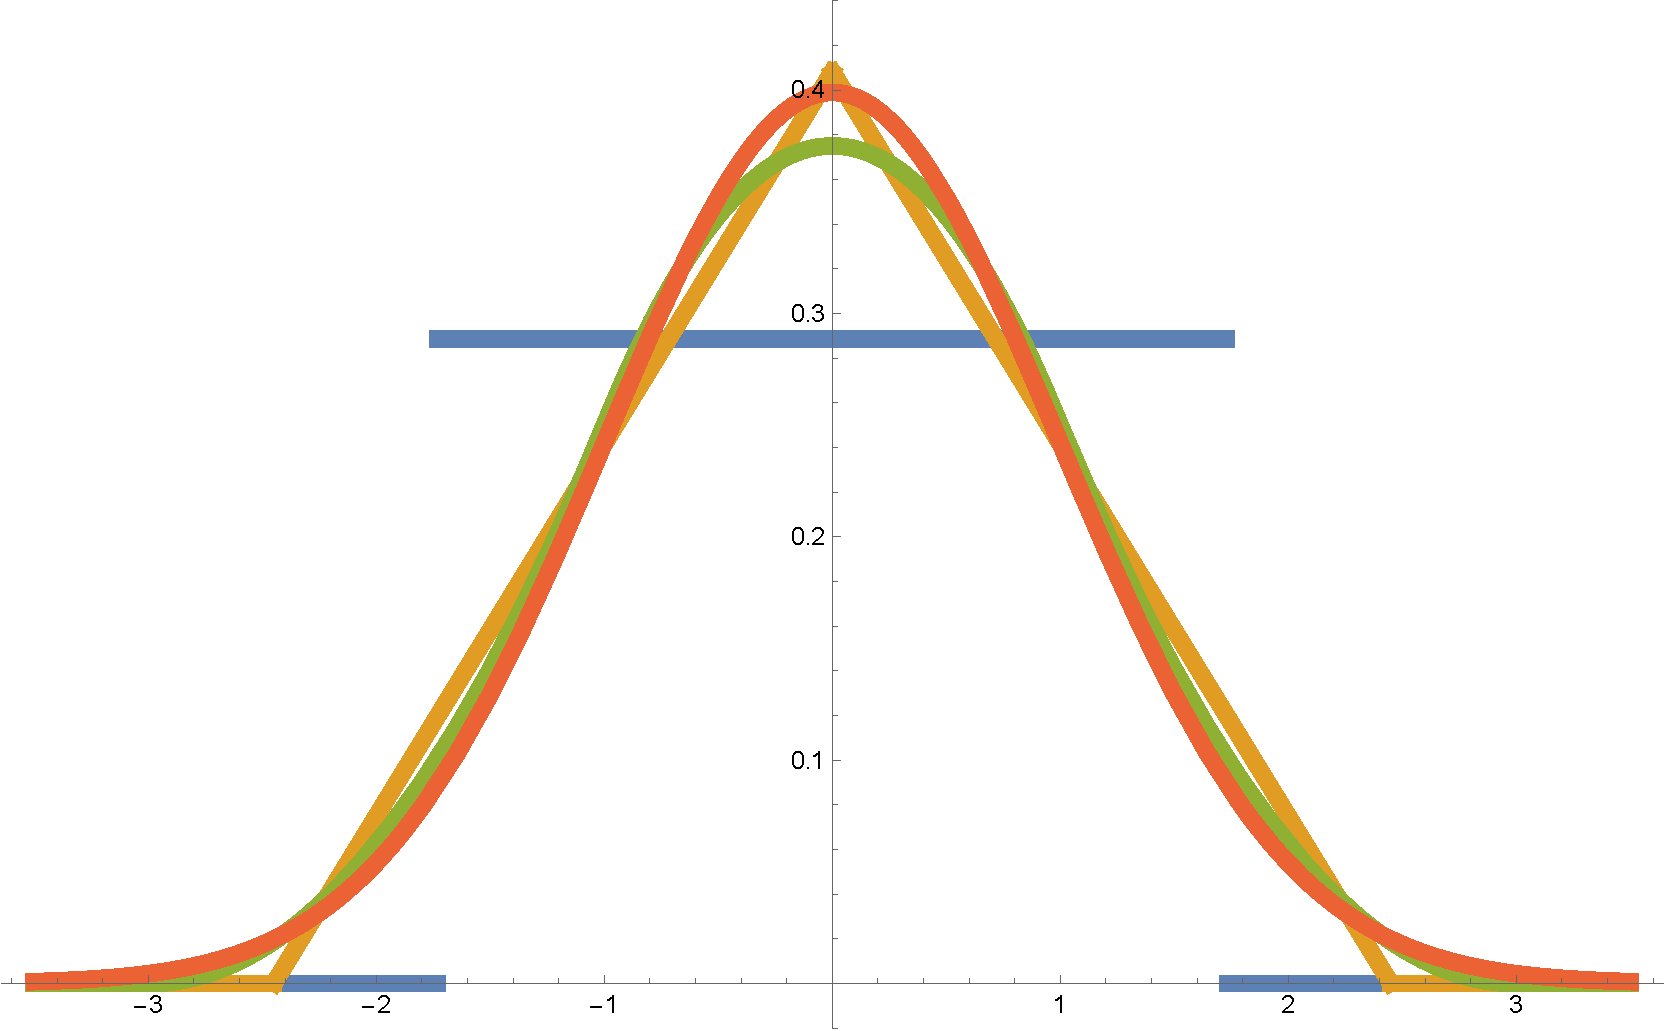
\includegraphics[width=0.5\textwidth]{./pictures/uniform_pdfs.pdf}
	\caption{Densities of $U_1$, $U_1+U_2$, $U_1+U_2+U_3$ (where $U_i$ are iid uniform on $[0,1]$),
		and $\mathcal{N}(0,1)$,
		normalized to have the same mean and variance.}
	\label{fig:uniform_pdfs}
\end{figure}

\begin{example}
Let $\{X_i\}_{i=1}^{\infty}$ be a sequence of iid Bernoulli random variables with parameter $p$, meaning that each $X_i$ takes the value $1$ with probability $p$ and $0$ with probability $1 - p$. The mean and variance of each $X_i$ are given by:
\[
	\mu = \operatorname{\mathbb{E}}[X_i] = p, \quad \sigma^2 = \operatorname{\mathrm{Var}}(X_i) = p(1 - p).
\]
We also have the distribution of $X_1+\cdots+X_n$:
\begin{equation*}
	\operatorname{\mathbb{P}}\left( X_1+ \cdots + X_n = k \right) = \binom{n}{k} p^k (1-p)^{n-k},
	\qquad k = 0, 1, \ldots, n.
\end{equation*}

Introduce the normalized quantity
\begin{equation}
	\label{eq:z_normalized_quantity}
	z = \frac{k - np}{\sqrt{np(1-p)}},
\end{equation}
and assume that throughout the asymptotic analysis,
this quantity stays finite.

Our aim is to show that, for $k$ such that $z$ remains bounded as $n\to\infty$, the following holds:
\[
\operatorname{\mathbb{P}}(S_n = k) = \frac{1}{\sqrt{2\pi np(1-p)}} \exp\Bigl( -\frac{z^2}{2} \Bigr) (1+o(1)).
\]

For large $n$, Stirling's formula gives
\[
m! \sim \sqrt{2\pi m}\, m^m e^{-m}, \quad \text{as } m\to\infty.
\]
Apply Stirling's approximation to $n!$, $k!$, and $(n-k)!$:
\[
n! \sim \sqrt{2\pi n}\, n^n e^{-n}, \quad
k! \sim \sqrt{2\pi k}\, k^k e^{-k}, \quad
(n-k)! \sim \sqrt{2\pi (n-k)}\,(n-k)^{n-k} e^{-(n-k)}.
\]
Thus,
\[
\binom{n}{k} \sim \frac{\sqrt{2\pi n}\, n^n e^{-n}}{\sqrt{2\pi k}\, k^k e^{-k}\sqrt{2\pi (n-k)}\,(n-k)^{n-k} e^{-(n-k)}}
= \frac{n^n}{k^k (n-k)^{n-k}}
\frac{1}{\sqrt{2\pi\, k(n-k)/n}}.
\]
More precisely, one often writes
\[
\binom{n}{k} \sim \frac{1}{\sqrt{2\pi np(1-p)}} \exp\Bigl( n\ln n - k\ln k - (n-k)\ln (n-k) \Bigr),
\]
where $p\approx k/n$ thanks to the fact that
$z$ \eqref{eq:z_normalized_quantity} is assumed to be finite.

We have
\[
k = np+ z\sqrt{np(1-p)}.
\]
Then, consider the second-order Taylor expansion. We have
\[
n\ln n - k\ln k - (n-k)\ln (n-k) \sim n H -\frac{z^2}{2},
\]
where $H=-[p\ln p+(1-p)\ln(1-p)]+c(z;p)/\sqrt n$
(for an explicit function $c(z;p)$)
is the
``entropy'' term which exactly cancels with the prefactors coming from $p^k (1-p)^{n-k}$.

After combining the approximations from the binomial coefficient and the probability weights, one arrives at
\[
\operatorname{\mathbb{P}}(S_n = k)
\sim \frac{1}{\sqrt{2\pi np(1-p)}} \exp\left( -\frac{z^2}{2} \right),
\]
as desired.


(Note that this is a \emph{local} CLT as opposed to the convergence
\eqref{eq:conv-in-dist} in the classical CLT; but one can get the latter
from the local CLT by integration.)

\end{example}


\subsection{Moments of the normal distribution}

\begin{proposition}
The moments of a random variable $Z \sim \mathcal{N}(0, \sigma^2)$ are given by:
\begin{equation}
	\label{eq:normal-moments}
	\operatorname{\mathbb{E}}[Z^k] = \begin{cases}
		0, & \text{if } k \text{ is odd}, \\
		\sigma^k (k-1)!! = \sigma^k \cdot (k-1)(k-3) \cdots 1, & \text{if } k \text{ is even}.
	\end{cases}
\end{equation}
\end{proposition}
\begin{proof}
	We just compute the integrals. Assume $k$ is even (for odd,
	the integral is zero by symmetry). Also assume $\sigma = 1$ for simplicity.
	Then
\begin{equation*}
	\operatorname{\mathbb{E}}[Z^k]
	=
	\frac{1}{\sqrt{2\pi}}
	\int_{-\infty}^{\infty}  z^k e^{-z^2/2} \, dz.
\end{equation*}
Applying integration by parts (putting $ze^{-z^2/2}$ under $d$), we get
\begin{equation*}
	\operatorname{\mathbb{E}}[Z^k] = \frac{1}{\sqrt{2\pi}} \left[-z^{k-1}e^{-z^2/2}\right]_{-\infty}^{\infty} + \frac{k-1}{\sqrt{2\pi}} \int_{-\infty}^{\infty} z^{k-2} e^{-z^2/2} \, dz.
\end{equation*}
The first term vanishes at infinity (you can verify this using L'Hôpital's rule), leaving us with:
\begin{equation*}
	\operatorname{\mathbb{E}}[Z^k] = (k-1)\operatorname{\mathbb{E}}[Z^{k-2}].
\end{equation*}
This gives us a recursive formula, and completes the proof.
\end{proof}


\subsection{Moments of sums of iid random variables}

Let us now show the CLT by moments.
For example, the source is
\cite[Section~30]{billingsley1995probability}
or \cite{filmus2010two}.


\begin{remark}
	This proof requires an additional assumption
	that all moments of the random variables are finite.
	This is quite a strong assumption, and while the CLT holds
	without it, this proof by moments is more algebraic, and
	will translate to random matrices more directly.
\end{remark}

\subsubsection{Computation of moments}

Denote $Y_i=X_i-\mu$, these are also iid, but have mean $0$.
We consider
\begin{equation*}
	\operatorname{\mathbb{E}}\left[ \left( \sum_{i=1}^n Y_i \right)^k \right].
\end{equation*}
Expanding the $k$-th power using the multinomial theorem, we obtain:
\begin{equation*}
\left( \sum_{i=1}^n Y_i \right)^k = \sum_{j_1 + j_2 + \dots + j_n = k}
Y_{j_1} Y_{j_2} \dots Y_{j_n}.
\end{equation*}
Taking the expectation and using linearity, we have:
\begin{equation*}
 \mathbb{E}\left[ \left( \sum_{i=1}^n Y_i \right)^k \right]
 =
 \sum_{j_1 + j_2 + \dots + j_n = k}
 \operatorname{\mathbb{E}}\left[
	 Y_{j_1} Y_{j_2} \dots Y_{j_n}
 \right].
\end{equation*}
The sum over all $j_1, \ldots, j_n$ with $j_1 + \ldots + j_n = k$ is the number of ways to partition $k$ into $n$ non-negative integers.
We can order these integers, and thus
obtain the sum over all partitions of $k$ into $\le n$ parts.
Since $n$ is large, we simply sum over all partitions of $k$.
For each partition $\lambda$ of $k$
(where $k=\lambda_1+\lambda_2+\ldots+\lambda_n $ and
$\lambda_1\geq \lambda_2\geq \ldots\geq \lambda_n\geq 0$),
we must count the number of distinct multisets of indices
\((j_1,j_2,\ldots,j_n)\) that yield the same collection
\(\{\lambda_1,\lambda_2,\ldots\}\).
Then,
\begin{equation*}
	\operatorname{\mathbb{E}}\left[
		Y_{j_1} Y_{j_2} \dots Y_{j_n}
	\right]=
	\mathsf{m}_{\lambda_1}\mathsf{m}_{\lambda_2}\ldots \mathsf{m}_{\lambda_n},
\end{equation*}
where $\mathsf{m}_j=\mathbb{E}[Y^j]$ (recall the identical distribution of $Y_i$).
Note that
$\mathsf{m}_0 = 1$ and
$\mathsf{m}_1 = 0$.
Let us illustrate this with an
example.

\begin{example}
	For $k=4$, there are only two partitions
	which have no parts equal to $1$:
	$\lambda=(4)$ and $\lambda=(2,2)$.
	The number of ways to get $(4)$
	(so that
	$\operatorname{\mathbb{E}}[Y_{j_1} Y_{j_2} Y_{j_3} Y_{j_4}] = \mathsf{m}_4$)
	is to just
	assign one of the $j_p$ to be $4$,
	this can be done in $n$ ways.

	The number of ways to get $(2,2)$
	(so that
	$\operatorname{\mathbb{E}}[Y_{j_1} Y_{j_2} Y_{j_3} Y_{j_4}] = \mathsf{m}_2^2$)
	is to assign
	two of the $j_p$ to be $2$ and the other two to be $0$, this can be done in $\binom{n}{2}$ ways. Moreover,
	there are also 6 permutations of the indices
	$j_p=(i,j)$ which give the same partition $(2,2)$:
	$(i,i,j,j)$, $(j,j,i,i)$, $(i,j,i,j)$, $(j,i,j,i)$, $(i,j,j,i)$, $(j,i,i,j)$.
	Thus, the total number of ways to get $(2,2)$ is $6\binom{n}{2}\sim 3n^2$.

	So, we see that there is an $n$-dependent factor,
	and a ``combinatorial'' factor for each partition.
\end{example}

\subsubsection{$n$-dependent factor}
\label{subsub:n-dependent-factor}

Consider first the $n$-dependent factor.
In the case $k$ is even and $\lambda=(2,2,\ldots,2 )$, the power
of $n$ is $n^{k/2}$.
In the case $k$ is even and $\lambda$ has at least one
part $\ge 3$, the power of $n$ is at most $n^{k/2-1}$,
which is subleading in the limit $n\to\infty$.
When $k$ is odd, the ``best'' we can do
(without parts equal to $1$)
is going to be
$\lambda=(3,2,\ldots, 2)$ with $(k-1)/2$ parts,
so the power of $n$ is $n^{(k-1)/2}$. This is also subleading
in the limit $n\to\infty$.


\subsubsection{Combinatorial factor}

Now, we see that we only need to consider the
case when $k$ is even and all parts of $\lambda$ are $2$.
Then, the $n$-dependent factor is $\binom{n}{k/2}\sim
n^{k/2}/(k/2)!$.
The combinatorial factor is
equal to the number of ways to partition $k$ into
pairs, which is the double factorial:
\begin{equation*}
	(k-1)!!=(k-1)(k-3)\ldots 1,
\end{equation*}
times the number of permutations
of the $k/2$ indices which are assigned to the pairs,
so $(k/2)!$.
In particular, for $k=4$ this is $6$.

\subsubsection{Putting it all together}

We have as $n\to\infty$:
\begin{equation*}
	\mathbb{E}\left[ \left( \sum_{i=1}^n Y_i \right)^k \right]
	=
	n^{k/2}
	\frac{(k-1)!!}{(k/2)!}\cdot (k/2)!
	\sigma^k
	+o(n^{k/2})=
	n^{k/2}
	(k-1)!!
	\sigma^k
	+o(n^{k/2}).
\end{equation*}

Now, we need to consider the normalization of the sum
$\sum_{i=1}^n Y_i$ by $\sqrt{n}$:
\begin{equation*}
	\mathbb{E}\left[ \left( \frac{1}{\sqrt{n}} \sum_{i=1}^n Y_i \right)^k \right]
	=
	\frac{1}{n^{k/2}}
	\mathbb{E}\left[ \left( \sum_{i=1}^n Y_i \right)^k \right]
	=
	(k-1)!!
	\sigma^k
	+o(1).
\end{equation*}
Therefore, the moments of
$Z_n$ \eqref{eq:normalized-sum}
converge to the moments of the standard normal distribution.


\subsection{Convergence in distribution}

Is convergence of moments enough to imply convergence in
distribution? Not necessarily. First, note that the functions
$x\mapsto x^k$ are not even bounded on $\mathbb{R}$.

A sufficient condition for convergence in distribution is
found in the
classical method of moments in
probability theory \cite[Theorem~30.2]{billingsley1995probability}.
This theorem
states that
if the limiting distribution $X$ is uniquely determined by its moments,
then convergence in moments implies convergence in distribution.

The normal distribution is indeed uniquely determined by its
moments (Problem \ref{prob:uniqueness-normal}),
so the CLT holds in this case, provided that the
original iid random variables $X_i$ have finite moments of
all orders.

\section{Random matrices and semicircle law}

We now turn to random matrices.

\subsection{Where can randomness in a matrix come from?}


The study of random matrices begins with understanding how randomness can be introduced into matrix structures. We consider three primary sources:
\begin{enumerate}
\item \textbf{iid entries:}
The simplest form of randomness comes from filling matrix entries independently with samples from a fixed probability distribution. For an $n \times n$ matrix, this gives us $n^2$ independent random variables.
If we do not impose any additional structure on the matrix, then the eigenvalues
will be complex. So, often we consider real symmetric, complex Hermitian, or quaternionic matrices with
symplectic symmetry.\footnote{Real symmetric means $A^\top=A$, complex Hermitian means $A^\dagger=A$ (conjugate transpose).
	Let us briefly discuss the quaternionic case. It can be modeled over $\mathbb{C}$. A quaternion
	$q = a + b\,\mathbf{i} + c\,\mathbf{j} + d\,\mathbf{k}$
	can be represented by the complex $2\times 2$ matrix
	\[
	q \;\longmapsto\;
	\begin{pmatrix}
	a + \mathbf{i}b & c + \mathbf{i}d \\
	-c + \mathbf{i}d & a - \mathbf{i}b
	\end{pmatrix}.
	\]
	The entries $a,b,c,d$ for the quaternion matrix case must be real, and the matrix
$A$ of size $2n\times 2n$ should also be Hermitian in the usual complex sense.\label{fn:quaternion}}


\item \textbf{Correlated Entries:}
In many physical systems, especially those modeling local interactions, matrix entries are not independent but show correlation patterns. Common examples include:
\begin{itemize}
\item Band matrices, where entries become negligible far from the diagonal
\item Matrices with correlation decay based on the distance between indices
\item Structured random matrices arising from specific physical models
\item Sparse matrices, where most entries are zero
\end{itemize}
\item \textbf{Haar Measure on Matrix Groups:}
Randomness can come from considering matrices sampled according to the Haar measure on compact matrix group,
for example, the orthogonal $O(n)$, unitary $U(n)$, or symplectic group $Sp(n)$.\footnote{The
	orthogonal and unitary groups are defined
	in the usual way, by $OO^\top=O^\top O=I$ and $UU^\dagger
	=U^\dagger U=I$, respectively.
	The
	group $Sp(n)$ is the compact real form of the full symplectic group $Sp(2n, \mathbb{C})$,
	consisting of $2n\times 2n$ matrices $A$ such that $A^\top JA=J$, where
	$J$ is the skew-symmetric form.}
One can think of this as a generalization of
the uniform distribution (Lebesgue measure) on the unit circle in $\mathbb{C}$,
or a unit sphere in $\mathbb{R}^n$.
One can also mix and match: one
of the most interesting families of random matrices is the one
with constant eigenvalues, but random eigenvectors:
\begin{equation*}
	A=UD_\lambda U^\dagger,\qquad U\in U(n), \quad U\sim \mathrm{Haar}.
\end{equation*}
Here $D_\lambda$ is a diagonal matrix with constant eigenvalues $\lambda=(\lambda_1,\ldots,\lambda_n)$.
The random matrix $A$ is the ``uniform'' random variable
taking values in the set of all Hermitian matrices with fixed real eigenvalues $\lambda$.
Here we may assume that $\lambda_1\ge \ldots\ge \lambda_n $,
since the unitary conjugation can permute the eigenvalues.
\end{enumerate}

\subsection{Real Wigner matrices}


\begin{definition}[Real Wigner Matrix]
An $n \times n$ random matrix $W=W_n = (X_{ij})_{1 \leq i,j \leq n}$ is called a \emph{real Wigner matrix} if:
\begin{enumerate}
    \item $W$ is symmetric: $X_{ij} = X_{ji}$ for all $i,j$;
    \item The upper triangular entries $\{X_{ij}: 1 \leq i \leq j \leq n\}$ are independent;
    \item The diagonal entries $\{X_{ii}\}$ are iid real random variables with mean $0$ and variance $\sigma_d$;
    \item The upper triangular entries $\{X_{ij}: i < j\}$ are iid
			(possibly with a distribution different from the diagonal entries) real random variables
			with mean $0$ and variance $\sigma$;
		\item (optional, but we assume this) All entries have finite moments of all orders.
\end{enumerate}
\end{definition}

\begin{example}[Gaussian Wigner Matrices, Gaussian Orthogonal Ensemble (GOE)]
Let $W$ be a real Wigner matrix where:
\begin{itemize}
    \item Diagonal entries $X_{ii} \sim \mathcal{N}(0, 2)$;
		\item Upper triangular entries $X_{ij} \sim \mathcal{N}(0, 1)$ for $i < j$.
\end{itemize}
We can model $W$ as $(Y+Y^\top)/\sqrt{2}$,
where $Y$ is a matrix with iid Gaussian entries $Y_{ij} \sim \mathcal{N}(0, 1)$.
The matrix distribution of $W$ is called
the \emph{Gaussian Orthogonal Ensemble} (\emph{GOE}).
\end{example}

\begin{remark}[Wishart Matrices]
	\label{rmk:wishart-matrices}
	There are other ways to define random matrices,
	most notably, \emph{sample covariance matrices}.
	Let $A = [a_{i,j}]_{i,j=1}^{n,m}$ be an $n \times m$ matrix ($n \leq m$), where entries are iid real random variables with
	mean $0$ and finite variance.
	Then $M = AA^\top$ is a positive symmetric random matrix of
	size $n \times n$. It almost surely has full rank.
\end{remark}


\subsection{Empirical spectral distribution}

For an arbitrary random matrix of size $n\times n$ with real eigenvalues,
the \emph{empirical spectral distribution} (\emph{ESD}) is defined as the
random probability measure on $\mathbb{R}$:
\begin{equation}
	\label{eq:esd-defintion}
	\mu_n = \frac{1}{n} \sum_{i=1}^n \delta_{\lambda_i},
\end{equation}
which puts point masses of size $1/n$ at the eigenvalues $\lambda_i$ of the matrix.

If you sample the ESD for a large real Wigner matrix,
and take a histogram (to cluster the eigenvalues into boxes),
you will see the semi-circular pattern. This pattern
does not change over several samples. Hence, one can
conjecture that the
ESD \eqref{eq:esd-defintion} converges to a nonrandom
measure, after rescaling.

We can guess the rescaling by looking at the first two moments of the ESD.
The first moment is
\begin{equation}
	\label{eq:first-moment-esd}
	\int_{\mathbb{R}} x \, \mu_n(dx) = \frac{1}{n} \sum_{i=1}^n \lambda_i=
	\frac{1}{n} \operatorname{Tr}(W) =
	\frac{1}{n}\sum_{i=1}^n X_{ii},
\end{equation}
and this sum has mean zero (and small variance), so it converges to zero.
The second moment is
\begin{equation}
	\label{eq:second-moment-esd}
	\int_{\mathbb{R}} x^2 \, \mu_n(dx) = \frac{1}{n} \sum_{i=1}^n \lambda_i^2=
	\frac{1}{n} \operatorname{Tr}(W^2) =
	\frac{1}{n}
	\sum_{i,j=1}^n X_{ij}^2.
\end{equation}
This sum has mean $\sim \sigma^2 n^2$, so even normalized by $n$,
it still goes to infinity.
But, if we normalize the matrix as $\frac{1}{\sqrt n}W$,
then the second moment
becomes bounded, and one can convince oneself that the
ESD of the normalized Wishart matrix has a limit.
Indeed, this is the case:

\begin{theorem}[Wigner's Semicircle Law]
	\label{thm:esd-semicircle}
	Let $W$ be a real Wigner matrix of size $n\times n$
	(with off-diagonal entries having a fixed variance $\sigma^2$, independent of $n$).
	Then
	as $n\to\infty$,
	the ESD of $W/(\sigma\sqrt{n})$ converges in distribution to the semicircular law:
	\begin{equation}
		\label{eq:thm-esd-semicircle}
		\nu_n\coloneqq \frac{1}{n}\sum_{i=1}^{n}\delta_{\lambda_i/\sqrt{n}}
		\longrightarrow \mu_{\mathrm{sc}},
	\end{equation}
	where $\mu_{\mathrm{sc}}$ is the semicircular distribution with density
	with respect to the Lebesgue measure:
	\begin{equation}
		\label{eq:semicircle-density-defintion}
		\mu_{\mathrm{sc}}(dx) \coloneqq \frac{1}{2\pi} \sqrt{4-x^2} \ssp \mathbf{1}_{|x| \leq 2}\ssp
		dx.
	\end{equation}
\end{theorem}

\begin{remark}
	The convergence in \eqref{eq:thm-esd-semicircle} may mean either
	\emph{weakly in probability} or \emph{weakly almost surely}.
	The first notion, weak convergence in probability, means that
	for every bounded continuous function $f$,
	we have
	\begin{equation}
		\label{eq:weak-convergence-in-prob}
		\int_{\mathbb{R}} f(x) \, \nu_n(dx) \longrightarrow \int_{\mathbb{R}} f(x) \, \mu_{\mathrm{sc}}(dx),\qquad  n\to\infty,
	\end{equation}
	where in \eqref{eq:weak-convergence-in-prob} the convergence is in probability.
	Indeed, the left-hand side of \eqref{eq:weak-convergence-in-prob}
	is a random variable, so we need to qualify which sense of convergence we mean.

	The weakly almost sure convergence means that
	the convergence in \eqref{eq:weak-convergence-in-prob}
	holds for almost all realizations of the random matrix $W$,
	that is, for every bounded continuous function $f$,
	the random variable
	$\int_{\mathbb{R}} f(x) \, \nu_n(dx)$ converges almost surely to
	$\int_{\mathbb{R}} f(x) \, \mu_{\mathrm{sc}}(dx)$.
\end{remark}

\begin{remark}
	There exists a version of the limiting
	ESD for the Wishart matrices
	(\Cref{rmk:wishart-matrices}).
	In this case, the limiting distribution is the
	\emph{Marchenko-Pastur law}
	\cite{MarchenkoPastur}.
\end{remark}

\subsection{Expected moments of traces of random matrices}

The main computation in the proof of
\Cref{thm:esd-semicircle} is the computation of
expected moments of the ESD.
This computation of moments is somewhat similar
to the one in the proof of the CLT by moments,
but has its own random matrix flavor.

\begin{definition}[Normalized Moments]
For each $k\geq 1$, the normalized $k$-th moment of the empirical spectral distribution of $W_n/\sqrt{n}$ is given by
\[
m_k^{(n)}=\int_{\mathbb{R}} x^k\,\nu_n(dx)
=\frac{1}{n^{k/2+1}}\operatorname{Tr}(W^k).
\]
\end{definition}
Our first goal is to study the asymptotic behavior of
$\operatorname{\mathbb{E}}[m_k^{(n)}]$ as $n\to\infty$ for each fixed
$k\geq 1$, just like we did in
\eqref{eq:first-moment-esd}--\eqref{eq:second-moment-esd}
for $k=1,2$:
\begin{equation*}
	\operatorname{\mathbb{E}}[m_1^{(n)}] = 0, \qquad
	\operatorname{\mathbb{E}}[m_2^{(n)}] \to \sigma^2.
\end{equation*}
Note that $\operatorname{\mathbb{E}}[m_2^{(n)}]$
is not exactly equal to $\sigma^2$ because of the presence of the
diagonal elements which have a different distribution.
In general, we will see that the contribution
of the diagonal elements to the moments is negligible
in the limit $n\to\infty$.

\begin{lemma}[Convergence of Expected Moments]
\label{lemma:moments_convergence}
For each fixed $k \geq 1$, we have
\[
\lim_{n \to \infty} \operatorname{\mathbb{E}}[m_k^{(n)}] =
\begin{cases}
0 & \text{if $k$ is odd}, \\
\sigma^k C_{k/2} & \text{if $k$ is even},
\end{cases}
\]
where $C_m = \frac{1}{m+1}\binom{2m}{m}$ is the $m$-th Catalan number.
\end{lemma}

The even moments are scaled by powers of $\sigma$ just as in the case $k=2$,
while the odd moments vanish due to the symmetry of the limiting distribution
around zero.
As we will see, the appearance of Catalan numbers is not accidental,
but it is due to the underlying combinatorics.

\begin{proof}[Proof of \Cref{lemma:moments_convergence}]
	The trace of $W^k$ expands as a sum over all possible index sequences:
	\begin{equation}
		\operatorname{Tr}(W^k) = \sum_{i_1,\ldots,i_k=1}^n X_{i_1i_2}X_{i_2i_3}\cdots X_{i_{k-1}i_k}X_{i_ki_1}.
	\end{equation}
	Due to independence and the fact that
	$\mathbb{E}[X_{ij}]=0$ for all $i,j$, the only nonzero
	contributions come from index sequences
	where each matrix element appears least twice.

	As in the CLT proof, there is a power-$n$ factor and a combinatorial factor.

	For $k$ odd, let us count the power of $n$ first. As
	in the CLT proof, the
	maximum power comes from index sequences where all matrix
	elements appear exactly twice except for one which appears
	three times. Indeed, this corresponds to the maximum
	freedom of choosing $k$ indices among the large number $n$
	of indices, and thus to the maximum power of $n$.
	This maximum power of $n$ is $n^{1+\lfloor k/2 \rfloor }$
	(note that there is an extra factor $n$ compared to the CLT proof,
	as now we have $\sim n^2$ random variables in the matrix instead of $n$).
	Since this is strictly less than the
	normalization $n^{k/2+1}$ in $m_k^{(n)}$, the term with odd $k$
	vanish in the limit $n\to\infty$.

	Assume now that $k$ is even.
	Then the maximum power of $n$ comes from index sequences where each matrix element appears exactly twice.
	This power of $n$ is $n^{k/2+1}$, which exactly
	matches the normalization in $m_k^{(n)}$.

	It remains to count the combinatorial factor,
	assuming that $k$ is even.
	For each term in the trace expansion, we can represent the sequence of indices $(i_1,\ldots,i_k)$ as a directed closed path with vertices $\{1,\ldots,n\}$ and edges given by the matrix entries $X_{i_ai_{a+1}}$. For example, if $k=4$ and we have a term $X_{12}X_{23}X_{34}X_{41}$, this corresponds to the path $1\to 2\to 3\to 4\to 1$. Recall that our path must have each
	matrix entry exactly twice (within the symmetry $X_{ij}=X_{ji}$),
	and the path must be closed.
	The condition that each edge appears exactly twice
	means that if we forget the direction of the edges and the multiplicities,
	we must get a \emph{tree}, with $k/2$ edges and $k/2+1$ vertices.
	The complete justification of this counting is the
	problem in Problem \ref{prob:counting-n-powers}.

	The $n$-powers counting implies that the combinatorial
	factor (for even $k$)
	is equal to $\sigma^k$ times the
	number of \emph{rooted} (\emph{planar}) \emph{trees} with $k/2$ edges.
	The rooted condition comes from the fact that
	we are free to choose fix the starting point of the path
	to be $1$ (this ambiguity is taken into account by the
	power-$n$ factor).

	In Problem \ref{prob:counting-trees}, we show that the number of these rooted trees is the $k/2$-th Catalan number $C_{k/2}$.
	This completes the proof of \Cref{lemma:moments_convergence}.
\end{proof}

\subsection{Immediate next steps}

The proof of \Cref{thm:esd-semicircle} is continued in the next
\href{https://lpetrov.cc/rmt25/rmt25-notes/rmt2025-l02.pdf}{Lecture 2}.
Immediate next steps are:
\begin{enumerate}
	\item Show that the number of rooted trees with $k/2$ edges is the $k/2$-th Catalan number, and give the exact formula for the Catalan numbers.
	\item Compute the moments of the semicircular distribution.
	\item Make sure that the moment computation suffice to show the
		weak in probability convergence of the ESD to the semicircular law.
\end{enumerate}


\appendix
\setcounter{section}{0}

\section{Problems (due 2025-02-13)}

Each problem is a subsection (like Problem \ref{prob:normal-approximation}),
and is may have several parts.

\subsection{Normal approximation}
\label{prob:normal-approximation}

\begin{enumerate}
	\item In \Cref{fig:uniform_pdfs}, which color is
		the normal curve and which is the sum of three uniform random variables?
	\item Show that the sum of 12 iid uniform random variables on $[-1,1]$
		(without normalization) is approximately standard normal.
	\item Find (numerically is okay)
		the maximum discrepancy between the distribution of the sum of 12 iid uniform random variables on $[-1,1]$ and the standard normal distribution:
		\begin{equation*}
			\sup_{x \in \mathbb{R}} \left| \operatorname{\mathbb{P}}\left(  \sum_{i=1}^{12} U_i \leq x \right) - \operatorname{\mathbb{P}}\left( Z \leq x \right) \right|.
		\end{equation*}
\end{enumerate}

\subsection{Convergence in distribution}
\label{prob:conv-in-dist-problem}

Convergence in distribution $X_n\to X$
for real random variables $X_n$ and $X$ means, by definition,
that
\begin{equation*}
	\operatorname{\mathbb{E}}[f(X_n)] \to \operatorname{\mathbb{E}}[f(X)]
\end{equation*}
for all bounded continuous functions $f$.
Show that convergence in distribution
is equivalent to the condition outlined in \eqref{eq:conv-in-dist}:
\begin{equation*}
	\lim_{n \to \infty} \operatorname{\mathbb{P}}(X_n \leq x) = \operatorname{\mathbb{P}}(X \leq x)
\end{equation*}
for all $x$ at which the cumulative distribution function of $X$ is continuous.

\subsection{Moments of sum justification}

Justify the computations of the power of $n$ in
\Cref{subsub:n-dependent-factor}.

\subsection{Distribution not determined by moments}

Show that the log-normal random variable
$e^{Z}$ (where $Z\sim \mathcal{N}(0,1)$)
is not determined by its moments.

\subsection{Uniqueness of the normal distribution}
\label{prob:uniqueness-normal}

Show that the normal distribution is uniquely determined by its moments.

\subsection{Quaternions}

Show that the $2\times 2$ matrix representation of a quaternion
given in Footnote~\ref{fn:quaternion}
indeed satisfies the quaternion multiplication rules.
Hint: Use linearity and distributive law.

\subsection{Ensemble $UD_\lambda U^\dagger$}

Let $U$ be the random Haar-distributed unitary matrix of size $N\times N$.
Let $D_\lambda$ be the diagonal matrix with constant real eigenvalues
$\lambda=(\lambda_1,\ldots,\lambda_N)$,
$\lambda_1\ge \ldots\ge \lambda_N$.
Let us fix $\lambda$ to be, say, $\lambda=(1,1,\ldots,1,0,0,\ldots,0  )$,
for some proportion of $1$'s and $0$'s (you can start with half
ones and half zeros).

Use a computer algebra system to
sample the eigenvalues of the matrix
obtained from $UD_\lambda U^\dagger$
by taking only its top-left corner of size $k\times k$,
where $k=1,2,\ldots,N $.
For a fixed $k$, let
$\lambda_1^{(k)}\ge \ldots\ge \lambda_k^{(k)}$
be the eigenvalues of the top-left corner of size $k\times k$.
Plot the two-dimensional array
\begin{equation*}
	\left\{ (\lambda_i^{(k)},k)\colon i=1,\ldots,k,\ k=1,\ldots,N  \right\}\subset \mathbb{R}\times
	\mathbb{Z}_{\ge1}.
\end{equation*}

\subsection{Invariance of the GOE}

Show that the distribution of the GOE is invariant under
conjugation by orthogonal matrices:
\begin{equation*}
	\operatorname{\mathbb{P}}(O W O^\top \in \mathrm{A}) = \operatorname{\mathbb{P}}(W \in \mathrm{A})
\end{equation*}
for all orthogonal matrices $O$ and Borel sets $\mathrm{A}$.

\subsection{Counting $n$-powers in the real Wigner matrix}
\label{prob:counting-n-powers}

Show that in the expansion of the expected trace of the
$k$-th power of the real Wigner matrix, the maximum power of
$n$ is $k/2+1$ for even $k$ and less for odd $k$. For even
$k$, the power $k/2+1$ comes from index sequences where each
off-diagonal matrix element appears exactly twice, and no
diagonal elements are present.





\subsection{Counting trees}
\label{prob:counting-trees}

Show that the number of rooted trees with $m$ edges is the $m$-th Catalan number:
\begin{equation*}
	C_m = \frac{1}{m+1}\binom{2m}{m}.
\end{equation*}






\bibliographystyle{alpha}
\bibliography{bib}


\medskip

\textsc{L. Petrov, University of Virginia, Department of Mathematics, 141 Cabell Drive, Kerchof Hall, P.O. Box 400137, Charlottesville, VA 22904, USA}

E-mail: \texttt{lenia.petrov@gmail.com}


\end{document}
